\section{Teilversuch 1: Bestimmung des Brechungsindex aus dem Reflexionskoeffizient für polarisiertes Licht}
	Wir berechnen zunächst den Fehler der einzelnen Multimetermessung mit:
	\begin{equation}
		\Delta I = 5\% \text{ Rdg} + 1 \text{ Dgt}
	\end{equation}
	\begin{beispiel}
		Für die erste Messung der Messreihe des senkrechten Fall:
		\begin{align}
			\SI{4.50}{\volt}\times\frac{0.5}{100} + \SI{0.01}{\volt} = \SI{0.0325}{\volt} = \SI{0.04}{\volt} \sigfig{1}
		\end{align}
	\end{beispiel}
	Die Normierung erhält man durch $\tilde{I} = \frac{I}{I_0}$ mit dem Fehler:
	\begin{align}
		\Delta \tilde{I} = \tilde{I}\relquad{I, I_0}
	\end{align}
	wobei $I$ und $I_0$ ensprechend mit $\nicefrac{1}{\text{Verstärkungsfaktor}}$ skaliert ist. Der Fehler der Eingangsintensitäten sind wegen Schwankungen während des Versuchs als $\Delta I_0 = \SI{0.05}{\volt}$ abgeschätzt. 
	\begin{beispiel}
		Für die erste Messung der Messreihe des senkrechten Fall:
		\begin{align}
			\tilde{I} &= \frac{\SI{4.50e-3}{\volt}}{\SI{1.23e-1}{\volt}} = \num{0.0365854} \sigfig{6} \\
			\Delta \tilde{I} &= 
			\frac{\SI{4.50e-3}{\volt}}{\SI{1.23e-1}{\volt}}\sqrt{
				\left(\frac{0.04}{4.50} \right)^2 +
				\left(\frac{0.05}{1.23} \right)^2
			} \notag \\
			&= \num{1.6e-3} \sigfig{2}
		\end{align}
		Somit erhalten wir $\tilde{I} = \num{0.366(16)}$.
	\end{beispiel}
	Um die Reflektionskoeffizienten zu erhalten müssen wir noch den Würzel ziehen ($\zeta = \sqrt{\tilde{I}}$) mit dem Fehler:
	\begin{align}
		\Delta \zeta = \gausserror{\zeta}{\tilde{I}} = \frac{\Delta \tilde{I}}{2\sqrt{\tilde{I}}}
	\end{align} Hier werden immer die genaue Werten von $\Delta \tilde{I}$ und $\tilde{I}$ verwendet, um Rundungsfehler zu vermeiden. 
	\begin{beispiel}
		Für die erste Messung der Messreihe des senkrechten Fall:
		\begin{align}
			\zeta &= \sqrt{\frac{\SI{4.50e-3}{\volt}}{\SI{1.23e-1}{\volt}}} = \num{0.191273} \sigfig{6} \\
			\Delta \zeta &= \frac{1}{2}
			\sqrt{\frac{\SI{4.50e-3}{\volt}}{\SI{1.23e-1}{\volt}}}\sqrt{
				\left(\frac{0.04}{4.50} \right)^2 +
				\left(\frac{0.05}{1.23} \right)^2
			} \notag \\
			&= \num{4e-3} \sigfig{1}
		\end{align}
		Somit erhalten wir $\zeta = \num{0.191(4)}$.
	\end{beispiel}

	Alle weitere Rechnung erfolgen im LibreOffice Calc. Rundung erfolgt mit der Funktion \texttt{ROUNDSIG} bzw. \texttt{ROUND}. 

	\subsection{Senkrechter Fall (Polarisationsfilter bei $\theta = \SI{0}{\degree}$)}
		Mit $\alpha = \frac{\varphi}{2}$:
		\begin{center}
			\begin{tabular}{@{} l  *{8}{l} @{}}
				\toprule
				$\alpha/\si{\degree}$        & \num{5.0} & \num{10.0} & \num{15.0} & \num{20.0} & \num{25.0} & \num{30.0} & \num{35.0} & \num{40.0} \\
				\midrule
				$I/\si{\volt}$               & \num{4.50} & \num{4.70} & \num{4.92} & \num{5.34} & \num{6.05} & \num{6.19} & \num{7.25} & \num{8.34} \\
				$\Delta I/\si{\volt}$        & \num{0.04} & \num{0.04} & \num{0.04} & \num{0.04} & \num{0.05} & \num{0.05} & \num{0.05} & \num{0.06} \\
				Verstärkung $/10^\square$    & \num{3} & \num{3} & \num{3} & \num{3} & \num{3} & \num{3} & \num{3} & \num{3} \\
				$\tilde{I}/\si{\volt}$       & \num{0.0366} & \num{0.0382} & \num{0.0400} & \num{0.0434} & \num{0.0492} & \num{0.0503} & \num{0.0589} & \num{0.0678} \\
				$\Delta\tilde{I}/\si{\volt}$ & \num{0.0016} & \num{0.0016} & \num{0.0017} & \num{0.0018} & \num{0.0021} & \num{0.0021} & \num{0.0025} & \num{0.0028} \\
				\midrule
				$\zeta^{\bot}$               & \num{0.191} & \num{0.195} & \num{0.200} & \num{0.208} & \num{0.222} & \num{0.224} & \num{0.243} & \num{0.260} \\
				$\Delta\zeta^{\bot}$         & \num{0.004} & \num{0.005} & \num{0.005} & \num{0.005} & \num{0.005} & \num{0.005} & \num{0.006} & \num{0.006} \\
				\bottomrule
				\\[-0.5em]
				\toprule
				$\alpha/\si{\degree}$        & \num{45.0} & \num{50.0} & \num{55.0} & \num{60.0} & \num{65.0} & \num{70.0} & \num{75.0} & \num{80.0} \\
				\midrule
				$I/\si{\volt}$               & \num{9.59} & \num{1.152} & \num{1.483} & \num{1.762} & \num{2.184} & \num{2.558} & \num{3.770} & \num{4.36} \\
				$\Delta I/\si{\volt}$        & \num{0.06} & \num{0.007} & \num{0.009} & \num{0.010} & \num{0.012} & \num{0.014} & \num{0.029} & \num{0.04} \\
				Verstärkung $/10^\square$    & \num{3} & \num{2} & \num{2} & \num{2} & \num{2} & \num{2} & \num{2} & \num{2} \\
				$\tilde{I}/\si{\volt}$       & \num{0.078} & \num{0.094} & \num{0.121} & \num{0.143} & \num{0.178} & \num{0.208} & \num{0.307} & \num{0.354} \\
				$\Delta\tilde{I}/\si{\volt}$ & \num{0.004} & \num{0.004} & \num{0.005} & \num{0.006} & \num{0.008} & \num{0.009} & \num{0.013} & \num{0.015} \\
				\midrule
				$\zeta^{\bot}$               & \num{0.279} & \num{0.306} & \num{0.347} & \num{0.378} & \num{0.421} & \num{0.456} & \num{0.554} & \num{0.595} \\
				$\Delta\zeta^{\bot}$         & \num{0.006} & \num{0.007} & \num{0.008} & \num{0.008} & \num{0.009} & \num{0.010} & \num{0.012} & \num{0.013} \\
				\bottomrule
			\end{tabular}
		\end{center}
		Es ist ein Fehler von $\Delta \alpha = \SI{2.5}{\degree}$ zu berücksichtigen.

		Nun tragen wir $\zeta^{\bot}$ gegen $\alpha$ und führe eine Kurveanpassung mit der (modifizierten) Gleichung (8) aus der Anleitung:
		\begin{equation}
			\zeta^{\bot} = \frac{\left(\sqrt{n^2 - \sin^2\alpha} - \cos\alpha\right)^2}{n^2 - 1}
		\end{equation}
		mittles \gnuplot{} durch (Siehe Appendix \ref{appdx:tv1-senk-gp}). Da die Brechungsindex $n$ von Flintglas definitv größer als $1$ ist, muss man hier die in Gleichung (8) stehende $1$ und $n^2$ im Nenner tauschen, sodass man positive Werte erhält. Als Anfangswert ist der Literaturwert\footnote{\href{https://www.rp-photonics.com/flint_glasses.html}{www.rp-photonics.com/flint\_glasses.html}} von $n=\num{1.55}$ verwendet. 
		\begin{figure}[H]
			\centering
			% GNUPLOT: LaTeX picture with Postscript
\begingroup
  \makeatletter
  \providecommand\color[2][]{%
    \GenericError{(gnuplot) \space\space\space\@spaces}{%
      Package color not loaded in conjunction with
      terminal option `colourtext'%
    }{See the gnuplot documentation for explanation.%
    }{Either use 'blacktext' in gnuplot or load the package
      color.sty in LaTeX.}%
    \renewcommand\color[2][]{}%
  }%
  \providecommand\includegraphics[2][]{%
    \GenericError{(gnuplot) \space\space\space\@spaces}{%
      Package graphicx or graphics not loaded%
    }{See the gnuplot documentation for explanation.%
    }{The gnuplot epslatex terminal needs graphicx.sty or graphics.sty.}%
    \renewcommand\includegraphics[2][]{}%
  }%
  \providecommand\rotatebox[2]{#2}%
  \@ifundefined{ifGPcolor}{%
    \newif\ifGPcolor
    \GPcolortrue
  }{}%
  \@ifundefined{ifGPblacktext}{%
    \newif\ifGPblacktext
    \GPblacktexttrue
  }{}%
  % define a \g@addto@macro without @ in the name:
  \let\gplgaddtomacro\g@addto@macro
  % define empty templates for all commands taking text:
  \gdef\gplbacktext{}%
  \gdef\gplfronttext{}%
  \makeatother
  \ifGPblacktext
    % no textcolor at all
    \def\colorrgb#1{}%
    \def\colorgray#1{}%
  \else
    % gray or color?
    \ifGPcolor
      \def\colorrgb#1{\color[rgb]{#1}}%
      \def\colorgray#1{\color[gray]{#1}}%
      \expandafter\def\csname LTw\endcsname{\color{white}}%
      \expandafter\def\csname LTb\endcsname{\color{black}}%
      \expandafter\def\csname LTa\endcsname{\color{black}}%
      \expandafter\def\csname LT0\endcsname{\color[rgb]{1,0,0}}%
      \expandafter\def\csname LT1\endcsname{\color[rgb]{0,1,0}}%
      \expandafter\def\csname LT2\endcsname{\color[rgb]{0,0,1}}%
      \expandafter\def\csname LT3\endcsname{\color[rgb]{1,0,1}}%
      \expandafter\def\csname LT4\endcsname{\color[rgb]{0,1,1}}%
      \expandafter\def\csname LT5\endcsname{\color[rgb]{1,1,0}}%
      \expandafter\def\csname LT6\endcsname{\color[rgb]{0,0,0}}%
      \expandafter\def\csname LT7\endcsname{\color[rgb]{1,0.3,0}}%
      \expandafter\def\csname LT8\endcsname{\color[rgb]{0.5,0.5,0.5}}%
    \else
      % gray
      \def\colorrgb#1{\color{black}}%
      \def\colorgray#1{\color[gray]{#1}}%
      \expandafter\def\csname LTw\endcsname{\color{white}}%
      \expandafter\def\csname LTb\endcsname{\color{black}}%
      \expandafter\def\csname LTa\endcsname{\color{black}}%
      \expandafter\def\csname LT0\endcsname{\color{black}}%
      \expandafter\def\csname LT1\endcsname{\color{black}}%
      \expandafter\def\csname LT2\endcsname{\color{black}}%
      \expandafter\def\csname LT3\endcsname{\color{black}}%
      \expandafter\def\csname LT4\endcsname{\color{black}}%
      \expandafter\def\csname LT5\endcsname{\color{black}}%
      \expandafter\def\csname LT6\endcsname{\color{black}}%
      \expandafter\def\csname LT7\endcsname{\color{black}}%
      \expandafter\def\csname LT8\endcsname{\color{black}}%
    \fi
  \fi
    \setlength{\unitlength}{0.0500bp}%
    \ifx\gptboxheight\undefined%
      \newlength{\gptboxheight}%
      \newlength{\gptboxwidth}%
      \newsavebox{\gptboxtext}%
    \fi%
    \setlength{\fboxrule}{0.5pt}%
    \setlength{\fboxsep}{1pt}%
\begin{picture}(8640.00,5760.00)%
    \gplgaddtomacro\gplbacktext{%
      \csname LTb\endcsname%%
      \put(814,704){\makebox(0,0)[r]{\strut{}$0,1$}}%
      \put(814,1332){\makebox(0,0)[r]{\strut{}$0,2$}}%
      \put(814,1960){\makebox(0,0)[r]{\strut{}$0,3$}}%
      \put(814,2588){\makebox(0,0)[r]{\strut{}$0,4$}}%
      \put(814,3215){\makebox(0,0)[r]{\strut{}$0,5$}}%
      \put(814,3843){\makebox(0,0)[r]{\strut{}$0,6$}}%
      \put(814,4471){\makebox(0,0)[r]{\strut{}$0,7$}}%
      \put(814,5099){\makebox(0,0)[r]{\strut{}$0,8$}}%
      \put(946,484){\makebox(0,0){\strut{}$0$}}%
      \put(1757,484){\makebox(0,0){\strut{}$10$}}%
      \put(2568,484){\makebox(0,0){\strut{}$20$}}%
      \put(3378,484){\makebox(0,0){\strut{}$30$}}%
      \put(4189,484){\makebox(0,0){\strut{}$40$}}%
      \put(5000,484){\makebox(0,0){\strut{}$50$}}%
      \put(5811,484){\makebox(0,0){\strut{}$60$}}%
      \put(6621,484){\makebox(0,0){\strut{}$70$}}%
      \put(7432,484){\makebox(0,0){\strut{}$80$}}%
      \put(8243,484){\makebox(0,0){\strut{}$90$}}%
    }%
    \gplgaddtomacro\gplfronttext{%
      \csname LTb\endcsname%%
      \put(209,2901){\rotatebox{-270}{\makebox(0,0){\strut{}Reflektionskoeffizient $\zeta^\bot$ (Einheitslos)}}}%
      \put(4594,154){\makebox(0,0){\strut{}Einfallswinkel $\alpha$ ($\si{\degree}$)}}%
      \csname LTb\endcsname%%
      \put(7256,1427){\makebox(0,0)[r]{\strut{}$\frac{\left(\sqrt{(1,46469)^2 - \sin^2\alpha} - \cos\alpha\right)^2}{(1,46469)^2 - 1}$}}%
      \csname LTb\endcsname%%
      \put(7256,987){\makebox(0,0)[r]{\strut{}Messpunkte}}%
      \csname LTb\endcsname%%
      \put(4594,5429){\makebox(0,0){\strut{}Reflektionskoeffizient gegen Einfallswinkel}}%
    }%
    \gplbacktext
    \put(0,0){\includegraphics[width={432.00bp},height={288.00bp}]{tv1-senkrecht}}%
    \gplfronttext
  \end{picture}%
\endgroup

			\caption{\centering Reflexionskoeffizient gegen Einfallswinkel $(\chi^2_{\text{red}} = 1.07006 \approx 1 \Rightarrow \text{Gute Anpassung})$ }
			\label{fig:tvone-senk}
			\vspace{-1em}
		\end{figure}
		Als Endergebnis erhalten wir $n = \num{1.46469(659)} = \num{1.465(7)}$. Aus dem Fit ist $\zeta^\bot$ bei senkrechtem Einfall ($\alpha = \SI{0}{\degree}$) gegeben durch:
		\begin{align}
			\zeta^\bot &= \frac{(n-1)^2}{n^2 - 1} = \frac{n - 1}{n + 1} = \frac{\num{1.465} - 1}{\num{1.465} + 1} = \num{0.188641} \sigfig{6} \\
			\Delta\zeta^\bot &= \gausserror{\zeta^{\bot}}{n} = \frac{(n+1)(1) - (n-1)(1)}{(n+1)^2}\Delta n \notag \\
			&= \frac{2\Delta n}{(n+1)^2} = \frac{2(\num{0.007})}{(\num{1.465}+1)^2} = \num{2.4e-3} \sigfig{2}
		\end{align}
		Also erhalten wir $\zeta^\bot(\SI{0}{\degree}) = \num{0.1886(24)}$. Es gibt hier keinen Minimum.

	\subsection{Paralleler Fall (Polarisationsfilter bei $\theta = \SI{90}{\degree}$)}
		Mit $\alpha = \frac{\varphi}{2}$:
		\begin{center}
			\begin{tabular}{@{} l  *{7}{l} @{}}
				\toprule
				$\alpha/\si{\degree}$        & \num{5.0} & \num{10.0} & \num{15.0} & \num{20.0} & \num{25.0} & \num{30.0} & \num{35.0} \\
				\midrule
				$I/\si{\volt}$               & \num{5.49} & \num{5.40} & \num{5.19} & \num{4.77} & \num{4.24} & \num{3.90} & \num{2.983} \\
				$\Delta I/\si{\volt}$        & \num{0.04} & \num{0.04} & \num{0.04} & \num{0.04} & \num{0.04} & \num{0.03} & \num{0.016} \\
				Verstärkung $/10^\square$    & \num{3} & \num{3} & \num{3} & \num{3} & \num{3} & \num{3} & \num{3} \\
				$\tilde{I}/\si{\volt}$       & \num{0.0416} & \num{0.0409} & \num{0.0393} & \num{0.0361} & \num{0.0321} & \num{0.0295} & \num{0.0226} \\
				$\Delta\tilde{I}/\si{\volt}$ & \num{0.0017} & \num{0.0016} & \num{0.0016} & \num{0.0015} & \num{0.0013} & \num{0.0012} & \num{0.0009} \\
				\midrule
				$\zeta^{\parallel}$          & \num{0.204} & \num{0.202} & \num{0.198} & \num{0.190} & \num{0.179} & \num{0.172} & \num{0.1503} \\
				$\Delta\zeta^{\parallel}$    & \num{0.004} & \num{0.004} & \num{0.004} & \num{0.004} & \num{0.004} & \num{0.004} & \num{0.0029} \\
				\bottomrule
				\\[-0.5em]
				\toprule
				$\alpha/\si{\degree}$        & \num{40.0} & \num{45.0} & \num{50.0} & \num{52.5} & \num{55.0} & \num{57.5} & \num{60.0} \\
				\midrule
				$I/\si{\volt}$               & \num{2.477} & \num{1.673} & \num{9.76} & \num{7.20} & \num{3.81} & \num{2.167} & \num{2.466} \\
				$\Delta I/\si{\volt}$        & \num{0.014} & \num{0.010} & \num{0.06} & \num{0.05} & \num{0.03} & \num{0.012} & \num{0.014} \\
				Verstärkung $/10^\square$    & \num{3} & \num{3} & \num{4} & \num{4} & \num{4} & \num{4} & \num{4} \\
				$\tilde{I}/\si{\volt}$       & \num{0.0188} & \num{0.0127} & \num{0.00739} & \num{0.00545} & \num{0.00289} & \num{0.00164} & \num{0.00187} \\
				$\Delta\tilde{I}/\si{\volt}$ & \num{0.0008} & \num{0.0005} & \num{0.00029} & \num{0.00022} & \num{0.00012} & \num{0.00007} & \num{0.00008} \\
				\midrule
				$\zeta^{\parallel}$          & \num{0.1370} & \num{0.1126} & \num{0.0860} & \num{0.0739} & \num{0.0537} & \num{0.0405} & \num{0.0432} \\
				$\Delta\zeta^{\parallel}$    & \num{0.0027} & \num{0.0022} & \num{0.0017} & \num{0.0015} & \num{0.0011} & \num{0.0008} & \num{0.0009} \\
				\bottomrule
				\\[-0.5em]
				\toprule
				$\alpha/\si{\degree}$        & \num{62.5} & \num{65.0} & \num{67.5} & \num{70.0} & \num{75.0} & \num{80.0} & \\
				\midrule
				$I/\si{\volt}$               & \num{4.59} & \num{9.85} & \num{1.907} & \num{4.11} & \num{1.008} & \num{1.677} & \\
				$\Delta I/\si{\volt}$        & \num{0.04} & \num{0.06} & \num{0.011} & \num{0.04} & \num{0.007} & \num{0.010} & \\
				Verstärkung $/10^\square$    & \num{4} & \num{4} & \num{3} & \num{3} & \num{2} & \num{2} & \\
				$\tilde{I}/\si{\volt}$       & \num{0.00348} & \num{0.00746} & \num{0.0144} & \num{0.0311} & \num{0.076} & \num{0.127} & \\
				$\Delta\tilde{I}/\si{\volt}$ & \num{0.00014} & \num{0.00029} & \num{0.0006} & \num{0.0013} & \num{0.003} & \num{0.005} & \\
				\midrule
				$\zeta^{\parallel}$          & \num{0.0590} & \num{0.0864} & \num{0.1202} & \num{0.176} & \num{0.276} & \num{0.356} & \\
				$\Delta\zeta^{\parallel}$    & \num{0.0012} & \num{0.0017} & \num{0.0024} & \num{0.004} & \num{0.006} & \num{0.007} & \\
				\bottomrule
			\end{tabular}
		\end{center}
		Es ist ein Fehler von $\Delta \alpha = \SI{2.5}{\degree}$ zu berücksichtigen.

		Wir bemerken zunächst, dass $\zeta^{\parallel}$ laut der Theorie je nach Einfallswinkel $\alpha$ unterschiedliche Vorzeichen haben. Um das Vorzeichen der experimentellen $\zeta^{\parallel}$-Werten bei dem Fit vernachlässigen zu können, tragen wir nun $\tilde{I} = \left(\zeta^{\parallel}\right)^2$ gegen $\alpha$ anstatt $\zeta^{\parallel}$ und führe eine Kurveanpassung mit der (modifizierten) Gleichung (9) aus der Anleitung:
		\begin{equation}
			\tilde{I} = \left(\zeta^{\parallel}\right)^2 = \left(\frac%
			{n^2\cos(\alpha) - \sqrt{n^2-\sin^2(\alpha)}}%
			{n^2\cos(\alpha) + \sqrt{n^2-\sin^2(\alpha)}}\right)^2
		\end{equation}
		mittles \gnuplot{} durch (Siehe Appendix \ref{appdx:tv1-parl-gp}). Als Anfangswert ist der Literaturwert\footnote{\href{https://www.rp-photonics.com/flint_glasses.html}{www.rp-photonics.com/flint\_glasses.html}} von $n=\num{1.55}$ verwendet. 
		\begin{figure}[H]
			\centering
			% GNUPLOT: LaTeX picture with Postscript
\begingroup
  \makeatletter
  \providecommand\color[2][]{%
    \GenericError{(gnuplot) \space\space\space\@spaces}{%
      Package color not loaded in conjunction with
      terminal option `colourtext'%
    }{See the gnuplot documentation for explanation.%
    }{Either use 'blacktext' in gnuplot or load the package
      color.sty in LaTeX.}%
    \renewcommand\color[2][]{}%
  }%
  \providecommand\includegraphics[2][]{%
    \GenericError{(gnuplot) \space\space\space\@spaces}{%
      Package graphicx or graphics not loaded%
    }{See the gnuplot documentation for explanation.%
    }{The gnuplot epslatex terminal needs graphicx.sty or graphics.sty.}%
    \renewcommand\includegraphics[2][]{}%
  }%
  \providecommand\rotatebox[2]{#2}%
  \@ifundefined{ifGPcolor}{%
    \newif\ifGPcolor
    \GPcolortrue
  }{}%
  \@ifundefined{ifGPblacktext}{%
    \newif\ifGPblacktext
    \GPblacktexttrue
  }{}%
  % define a \g@addto@macro without @ in the name:
  \let\gplgaddtomacro\g@addto@macro
  % define empty templates for all commands taking text:
  \gdef\gplbacktext{}%
  \gdef\gplfronttext{}%
  \makeatother
  \ifGPblacktext
    % no textcolor at all
    \def\colorrgb#1{}%
    \def\colorgray#1{}%
  \else
    % gray or color?
    \ifGPcolor
      \def\colorrgb#1{\color[rgb]{#1}}%
      \def\colorgray#1{\color[gray]{#1}}%
      \expandafter\def\csname LTw\endcsname{\color{white}}%
      \expandafter\def\csname LTb\endcsname{\color{black}}%
      \expandafter\def\csname LTa\endcsname{\color{black}}%
      \expandafter\def\csname LT0\endcsname{\color[rgb]{1,0,0}}%
      \expandafter\def\csname LT1\endcsname{\color[rgb]{0,1,0}}%
      \expandafter\def\csname LT2\endcsname{\color[rgb]{0,0,1}}%
      \expandafter\def\csname LT3\endcsname{\color[rgb]{1,0,1}}%
      \expandafter\def\csname LT4\endcsname{\color[rgb]{0,1,1}}%
      \expandafter\def\csname LT5\endcsname{\color[rgb]{1,1,0}}%
      \expandafter\def\csname LT6\endcsname{\color[rgb]{0,0,0}}%
      \expandafter\def\csname LT7\endcsname{\color[rgb]{1,0.3,0}}%
      \expandafter\def\csname LT8\endcsname{\color[rgb]{0.5,0.5,0.5}}%
    \else
      % gray
      \def\colorrgb#1{\color{black}}%
      \def\colorgray#1{\color[gray]{#1}}%
      \expandafter\def\csname LTw\endcsname{\color{white}}%
      \expandafter\def\csname LTb\endcsname{\color{black}}%
      \expandafter\def\csname LTa\endcsname{\color{black}}%
      \expandafter\def\csname LT0\endcsname{\color{black}}%
      \expandafter\def\csname LT1\endcsname{\color{black}}%
      \expandafter\def\csname LT2\endcsname{\color{black}}%
      \expandafter\def\csname LT3\endcsname{\color{black}}%
      \expandafter\def\csname LT4\endcsname{\color{black}}%
      \expandafter\def\csname LT5\endcsname{\color{black}}%
      \expandafter\def\csname LT6\endcsname{\color{black}}%
      \expandafter\def\csname LT7\endcsname{\color{black}}%
      \expandafter\def\csname LT8\endcsname{\color{black}}%
    \fi
  \fi
    \setlength{\unitlength}{0.0500bp}%
    \ifx\gptboxheight\undefined%
      \newlength{\gptboxheight}%
      \newlength{\gptboxwidth}%
      \newsavebox{\gptboxtext}%
    \fi%
    \setlength{\fboxrule}{0.5pt}%
    \setlength{\fboxsep}{1pt}%
\begin{picture}(8640.00,5760.00)%
    \gplgaddtomacro\gplbacktext{%
      \csname LTb\endcsname%%
      \put(946,704){\makebox(0,0)[r]{\strut{}$0$}}%
      \put(946,1332){\makebox(0,0)[r]{\strut{}$0,05$}}%
      \put(946,1960){\makebox(0,0)[r]{\strut{}$0,1$}}%
      \put(946,2588){\makebox(0,0)[r]{\strut{}$0,15$}}%
      \put(946,3215){\makebox(0,0)[r]{\strut{}$0,2$}}%
      \put(946,3843){\makebox(0,0)[r]{\strut{}$0,25$}}%
      \put(946,4471){\makebox(0,0)[r]{\strut{}$0,3$}}%
      \put(946,5099){\makebox(0,0)[r]{\strut{}$0,35$}}%
      \put(1078,484){\makebox(0,0){\strut{}$0$}}%
      \put(1874,484){\makebox(0,0){\strut{}$10$}}%
      \put(2670,484){\makebox(0,0){\strut{}$20$}}%
      \put(3466,484){\makebox(0,0){\strut{}$30$}}%
      \put(4262,484){\makebox(0,0){\strut{}$40$}}%
      \put(5059,484){\makebox(0,0){\strut{}$50$}}%
      \put(5855,484){\makebox(0,0){\strut{}$60$}}%
      \put(6651,484){\makebox(0,0){\strut{}$70$}}%
      \put(7447,484){\makebox(0,0){\strut{}$80$}}%
      \put(8243,484){\makebox(0,0){\strut{}$90$}}%
    }%
    \gplgaddtomacro\gplfronttext{%
      \csname LTb\endcsname%%
      \put(209,2901){\rotatebox{-270}{\makebox(0,0){\strut{}Reflektionskoeffizient$^2$ $\left(\zeta^\parallel\right)^2$ (Einheitslos)}}}%
      \put(4660,154){\makebox(0,0){\strut{}Einfallswinkel $\alpha$ ($\si{\degree}$)}}%
      \csname LTb\endcsname%%
      \put(7256,4816){\makebox(0,0)[r]{\strut{}$\left(\frac{(1,52605)^2\cos(\alpha) - \sqrt{(1,52605)^2-\sin^2(\alpha)}}{(1,52605)^2\cos(\alpha) + \sqrt{(1,52605)^2-\sin^2(\alpha)}}\right)^2$}}%
      \csname LTb\endcsname%%
      \put(7256,4376){\makebox(0,0)[r]{\strut{}Messpunkte}}%
      \csname LTb\endcsname%%
      \put(4660,5429){\makebox(0,0){\strut{}Reflektionskoeffizient$^2$ gegen Einfallswinkel}}%
    }%
    \gplbacktext
    \put(0,0){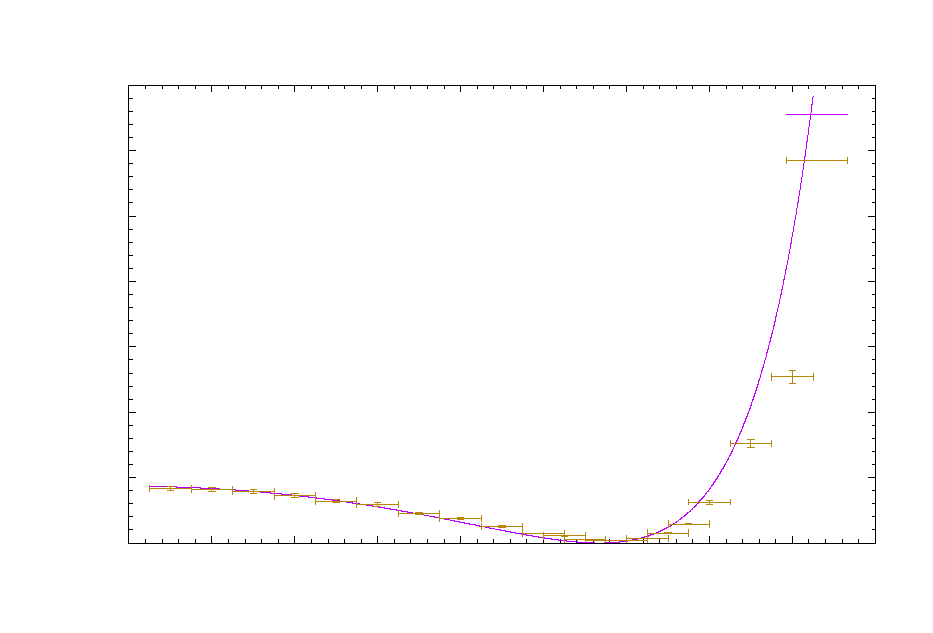
\includegraphics[width={432.00bp},height={288.00bp}]{tv1-parallel}}%
    \gplfronttext
  \end{picture}%
\endgroup

			\caption{\centering Reflexionskoeffizient$^2$ gegen Einfallswinkel $(\chi^2_{\text{red}} = 1.58636 \approx 1 \Rightarrow \text{Gute Anpassung})$ }
			\label{fig:tvone-parl}
			\vspace{-1em}
		\end{figure}
		Als Endergebnis erhalten wir $n = \num{1.52605(879)} = \num{1.526(9)}$. Aus dem Fit ist $\zeta^\parallel$ bei senkrechtem Einfall ($\alpha = \SI{0}{\degree}$) gegeben durch:
		\begin{align}
			\zeta^\parallel &= \frac%
			{n^2 - n}%
			{n^2 + n} 
			= \frac{n-1}{n+1} = \frac{\num{1.526} - 1}{\num{1.526} + 1} = \num{0.208234} \sigfig{6}\\
			\Delta\zeta^\parallel &= \gausserror{\zeta^{\bot}}{n} = \frac{(n+1)(1) - (n-1)(1)}{(n+1)^2}\Delta n \notag \\
			&= \frac{2\Delta n}{(n+1)^2} = \frac{2(\num{0.009})}{(\num{1.526}+1)^2} = \num{2.9e-3} \sigfig{2}
		\end{align}
		Also erhalten wir $\zeta^\parallel(\SI{0}{\degree}) = \num{0.2082(29)}$. Da es schwer ist, um das Minimum aus dem Graphik abzulesen, verwenden wir WolframAlpha\footnote{\href{https://www.wolframalpha.com/input/?i=minimum+of+\%28\%281.526*1.526*cos\%28x\%29-sqrt\%281.526*1.526+-+sin\%28x\%29*sin\%28x\%29\%29\%29+\%2F+\%281.526*1.526*cos\%28x\%29\%2Bsqrt\%281.526*1.526+-+sin\%28x\%29*sin\%28x\%29\%29\%29\%29**2+with+x+from+0+to+1.57}{https://www.wolframalpha.com/input/?i=minimum of ((1.526*1.526*cos(x)-sqrt(1.526*1.526 - sin(x)*sin(x))) / (1.526*1.526*cos(x)+sqrt(1.526*1.526 - sin(x)*sin(x))))**2 with x from 0 to 1.57}}. 

		Wir erhalten somit den Wert $\alpha_p = \SI{0.990699}{\radian} = \SI{56.8}{\degree}$. Es war leider zeitlich schwer, mit dieser Methode auch den Fehler von $\alpha_p$ zu bestimmen. Dazu muss man erst herausfinden, was für ein Effekt die Variation von $n$ auf dem Ergebnis hat. 

		Das gemessene Minimum war bei $\alpha_p = \SI{57.5(25)}{\degree}$. Dieser Wert stimmt mit dem Minimum aus dem Fit überein und der Brechungsindex (und dessen Fehler) daraus ist gegeben durch:
		\begin{align}
			n &= \tan(\alpha_p) = \tan{\SI{57.5}{\degree}/\si{\degree}} = \num{1.56969} \sigfig{6} \\
			\Delta n &= \gausserror{n}{\alpha_p} = (\Delta\alpha_p)\sec^2{\alpha_p} =\frac{\Delta\alpha_p}{\cos^2\alpha_p} \notag \\
			&= \frac{2.5 \cdot \frac{\pi}{180}}{\cos^2(\SI{57.5}{\degree}/\si{\degree})} = \num{0.16} \sigfig{2}
		\end{align}
		Somit erhalten wir $n = \num{1.57(16)}$.
	\subsection{Diskussion}
		Wir berechenen zunächst aus der angegebenen Reflexionskoeffizienten in Tabelle 1 der Anleitung die theoretische Berechungsindex des Flintglases. Es gilt beim senkrechten Einfall ($\alpha = \SI{0}{\degree}$), dass:
		\begin{align}
			\zeta^\parallel = \zeta^\bot = \frac{n-1}{n+1} &= \num{0.240} \notag\\
			n-1 &= \num{0.240}\left(n+1\right) \notag \\
			n(1-\num{0.240}) &= 1+ \num{0.240} \notag \\
			n &= \frac{1+ \num{0.240}}{1 -\num{0.240}} = 1.63 \sigfig{3}
		\end{align}
		Zusammengefasst haben wir aus unseren Ergebnisse vom Teilversuch 1:
		\begin{center}
			\begin{tabular}{ll}
				\toprule
				Methode & $n$ \\
				\midrule
				$\zeta^\bot$      & \num{1.465(7)} \\
				$\zeta^\parallel$ & \num{1.526(9)} \\
				$\alpha_p$        & \num{1.57(16)} \\
				\midrule
				Anleitung         & \num{1.63} \\
				\bottomrule
			\end{tabular}
		\end{center}
		Die experimentelle Werten stimmen miteinander überein, aber nur $n$ aus $\alpha_p$ ist mit der Literaturwert aus der Anleitung verträglich. Hierfür verwenden wir nicht den Literaturwert aus dem Internet, da die Brechungsindizes von Flintgläsern je nach Materie sehr unterschiedlich sind. Wir gehen somit davon aus, dass der Wert aus der Anleitung das richtige Flintglas entspricht. 

		Der Unterschied zwischen den Literaturwert und den experimentell gemessenenen Wert kann vermütlich an den folgenden Fehlerquellen liegen:
		\begin{itemize}
			\item Der Laserstrahl war nicht komplett horizontal, was die Richtung der Polarisation im Vergleich zur Reflektionsebene ändern könnten. Das heißt, dass der senkrechten bzw. parallelen Fall nicht wirklich senkrecht und parallel sind. Das hat zur Folge, dass die Fresnelsche Gleichung nicht komplett anwendbar waren. 
			\item Das Licht im Raum war hell und könnten zur Fehler bei der Messungen führen. Obwohl wir die Nullausgleich gemacht haben, ist der Beitrag von der Raumbeleuchtung je nach Ausrichtung des Prismas unterschiedlich. Da die Beleuchtung auch durch Reflexion polarisiert werden kann, könnte es bei kleiner Messwerten (besonders mit $10^3$ oder $10^4$ Verstärkungen) einen großen Einfluss haben.
			\item Die Polarisationsfilter sind auch nicht perfekt. Wenn die beide Polarisatoren senkrecht stehen, gibt es immer noch ein bisschen Licht, das durch kommt. Dieses Effekt war während des Versuchs leider nicht charakterisiert und deswegen wissen auch nicht, wie dieses Effekt zur unseren Ergebnissen beigetragen haben.
		\end{itemize}
